% Options for packages loaded elsewhere
\PassOptionsToPackage{unicode}{hyperref}
\PassOptionsToPackage{hyphens}{url}
\documentclass[
  11pt,
  letterpaper,
]{article}
\usepackage{xcolor}
\usepackage[margin=1in]{geometry}
\usepackage{authblk}
\usepackage{float}
\usepackage{amsmath,amssymb}
\setcounter{secnumdepth}{-\maxdimen} % remove section numbering
\usepackage{iftex}
\ifPDFTeX
  \usepackage[T1]{fontenc}
  \usepackage[utf8]{inputenc}
  \usepackage{textcomp} % provide euro and other symbols
  \DeclareUnicodeCharacter{03B2}{\ensuremath{\beta}}
\else % if luatex or xetex
  \usepackage{unicode-math} % this also loads fontspec
  \defaultfontfeatures{Scale=MatchLowercase}
  \defaultfontfeatures[\rmfamily]{Ligatures=TeX,Scale=1}
\fi
\usepackage{lmodern}
\ifPDFTeX\else
  % xetex/luatex font selection
\fi
% Use upquote if available, for straight quotes in verbatim environments
\IfFileExists{upquote.sty}{\usepackage{upquote}}{}
\IfFileExists{microtype.sty}{% use microtype if available
  \usepackage[]{microtype}
  \UseMicrotypeSet[protrusion]{basicmath} % disable protrusion for tt fonts
}{}
\makeatletter
\@ifundefined{KOMAClassName}{% if non-KOMA class
  \IfFileExists{parskip.sty}{%
    \usepackage{parskip}
  }{% else
    \setlength{\parindent}{0pt}
    \setlength{\parskip}{6pt plus 2pt minus 1pt}}
}{% if KOMA class
  \KOMAoptions{parskip=half}}
\makeatother
\usepackage{longtable,booktabs,array,tabularx}
\newcounter{none} % for unnumbered tables
\usepackage{calc} % for calculating minipage widths
% Correct order of tables after \paragraph or \subparagraph
\usepackage{etoolbox}
\makeatletter
\patchcmd\longtable{\par}{\if@noskipsec\mbox{}\fi\par}{}{}
\makeatother
% Allow footnotes in longtable head/foot
\IfFileExists{footnotehyper.sty}{\usepackage{footnotehyper}}{\usepackage{footnote}}
\makesavenoteenv{longtable}
\usepackage{graphicx}
\usepackage{placeins}
\usepackage[
  backend=biber,
  style=authoryear,
  sorting=nyt,
  maxcitenames=2,
  mincitenames=1,
  maxbibnames=6,
  minbibnames=3,
  giveninits=true,
  uniquename=false,
  date=year,
  doi=true,
  url=true,
  isbn=false
]{biblatex}
\addbibresource{grasb.bib}
\DeclareDelimFormat{nameyeardelim}{\addcomma\space}
\setlength{\bibitemsep}{0.7\baselineskip}
\AtEveryBibitem{%
  \clearfield{month}%
  \clearfield{day}%
  \clearfield{urlyear}%
  \clearfield{urlmonth}%
  \clearfield{urlday}%
  \clearfield{langid}%
  \clearlist{language}%
  \iffieldundef{doi}{}{\clearfield{url}}%
}
\makeatletter
\newsavebox\pandoc@box
\newcommand*\pandocbounded[1]{% scales image to fit in text height/width
  \sbox\pandoc@box{#1}%
  \Gscale@div\@tempa{\textheight}{\dimexpr\ht\pandoc@box+\dp\pandoc@box\relax}%
  \Gscale@div\@tempb{\linewidth}{\wd\pandoc@box}%
  \ifdim\@tempb\p@<\@tempa\p@\let\@tempa\@tempb\fi% select the smaller of both
  \ifdim\@tempa\p@<\p@\scalebox{\@tempa}{\usebox\pandoc@box}%
  \else\usebox{\pandoc@box}%
  \fi%
}
% Set default figure placement to htbp
\def\fps@figure{htbp}
\makeatother
\setlength{\emergencystretch}{3em} % prevent overfull lines
\providecommand{\tightlist}{%
  \setlength{\itemsep}{0pt}\setlength{\parskip}{0pt}}
\usepackage{bookmark}
\IfFileExists{xurl.sty}{\usepackage{xurl}}{} % add URL line breaks if available
\urlstyle{same}
\hypersetup{
  pdftitle={GRASB: Gene-Regulatory Alignment of Schrödinger Bridges for Single-Cell Trajectories in Latent Space},
  hidelinks,
  pdfcreator={LaTeX via pandoc}}

\title{GRASB: Gene-Regulatory Alignment of Schrödinger Bridges for
Single-Cell Trajectories in Latent Space}
\author[1,2]{First Author}
\author[1,2]{Second Author}
\affil[1]{First affiliation}
\affil[2]{Second affiliation}
\date{}

\begin{document}
\maketitle
\begin{NoHyper}
\begingroup
\renewcommand{\thefootnote}{}
\footnotetext{This manuscript describes ongoing work.}
\endgroup
\end{NoHyper}
\begin{abstract}
Time-series single-cell RNA sequencing observes population snapshots,
but the cell lysis required for sequencing prevents individual cells
from being followed over time. Schrödinger bridges infer continuous
stochastic transport between these snapshots, often in latent
representations that provide denoising but make the regulatory meaning
of the learned dynamics difficult to interpret. We introduce
Gene-Regulatory Alignment of Schrödinger Bridges (GRASB), a
gene-regulatory-network-guided unbalanced Schrödinger bridge that couples
gene-resolved regulatory information to latent transport. To solve this,
we define a cell-contextualized transcription factor--target
velocity in gene space, map it through the encoder of a frozen
variational autoencoder using a Jacobian--vector product to guide the
latent bridge, and map the learned drift back through the decoder.
To test whether the resulting alignment depends on regulatory topology,
we compare GRASB with matched unguided and degree-preserving
shuffled-network controls. In the datasets tested, genuine network
guidance yields decoded-drift genes that are more enriched for the
corresponding cell-type and lineage programs than both controls. The
results reveal a useful trade-off for applications that prioritize
biological interpretability over distributional fidelity. Code is available at
\texttt{[repository URL]}.
\end{abstract}

\section{1. Introduction}\label{introduction}

Single-cell RNA sequencing (scRNA-seq) measures cells destructively, so
time-series experiments observe different cells at each timepoint.
Trajectory-inference methods recover developmental order and topology
from transcriptional similarity \parencite{saelens_comparison_2019}, while optimal
transport methods couple population snapshots and can account for growth
and death \parencite{schiebinger_optimal-transport_2019}. Schrödinger bridges (SBs) extend
this population view to distributions over continuous stochastic paths.
Neural solvers have made this formulation practical for high-dimensional
cell dynamics, including unbalanced settings in which population mass
changes over time \parencite{de_bortoli_diffusion_2021,pariset_unbalanced_2023,
alatkar_artemis_2025,zhang_modeling_2025}.

Because gene-expression measurements are high dimensional, these models
often learn transport in a denoised latent representation. This reduces
computational cost, but the representation combines signals from many
genes. A decoder can map latent drift back to named genes, yet a recognizable
gene ranking does not show that the dynamics follow regulatory programs
specific to a cell type or lineage. Moreover, local decoded drift and
generated expression answer different questions: drift is an
instantaneous direction, whereas generated states integrate drift,
diffusion, and population birth or death. Biological organization of the
vector field may therefore differ from fidelity of the reconstructed
population.

Gene regulatory networks (GRNs) provide a complementary source of
biological structure by preserving explicit transcription-factor
(TF)--target relationships in gene space \parencite{aibar_scenic_2017}.
Context-specific linear models can assign signed coefficients to
candidate edges and thereby define a
regulatory direction at an observed cell state \parencite{kamimoto_dissecting_2023}.
Combining these models creates a representational mismatch: applying a
GRN directly to latent features discards gene identity, whereas learning
transport in full expression space sacrifices the advantages of the
latent representation.

We bridge the two representations with Gene-Regulatory Alignment of
Schrödinger Bridges (GRASB), which transports a regulatory velocity
rather than the network itself. A frozen VAE encoder maps a
cell-contextualized gene-space velocity into the latent bridge through a
Jacobian--vector product (JVP); after training, a decoder JVP maps latent
drift back to signed gene velocities. The GRN acts as a soft prior rather
than as causal ground truth. We test the method in human pancreatic endocrine
differentiation and zebrafish embryogenesis
\parencite{veres_charting_2019,farrell_single-cell_2018}. Genuine GRN guidance improves alignment of decoded
drift with lineage programs relative to unguided and degree-preserving
shuffled-network controls, but worsens held-out population fit. These
results motivate separate evaluation of local vector-field biology and
integrated trajectory fidelity.

\section{2. Related work}\label{related-work}

\subsection{2.1 Schrödinger bridges for cell
dynamics}\label{sbs-for-cell-dynamics}

An SB finds a path measure that matches specified endpoint distributions
while minimizing relative entropy to a reference stochastic process
\parencite{schrodinger_sur_1932,leonard_schrodinger_2012}. For Brownian reference dynamics, its
static form is entropy-regularized quadratic OT and converges to
quadratic OT as diffusivity vanishes \parencite{carlier_convergence_2017}.
Computationally, iterative proportional fitting (IPF) enforces the
endpoint marginals and reduces to Sinkhorn scaling for discrete measures
\parencite{cuturi_sinkhorn_2013}. Sample-based extensions replace a fixed spatial grid with
regression, likelihood, or importance-sampling updates
\parencite{bernton_schrodinger_2019,pavon_data-driven_2021,vargas_solving_2021}.

Neural diffusion SBs continue this progression by learning forward and
reverse drifts from simulated paths, which enables minibatched training
in high dimensions \parencite{de_bortoli_diffusion_2021,chen_likelihood_2021}.
Standard SBs nevertheless conserve mass, whereas cell populations change
through proliferation and death. Unbalanced OT introduces mass variation
\parencite{chizat_interpolating_2018,liero_optimal_2018}, and unbalanced Schrödinger
bridges (uSBs) incorporate it into the stochastic path law through
killing and time-reversed birth
\parencite{chen_most_2022,pariset_unbalanced_2023}. Within single-cell analysis,
Waddington-OT estimates couplings between sampled times using growth information
\parencite{schiebinger_optimal-transport_2019}; ARTEMIS combines a VAE with a uSB for
continuous multi-timepoint trajectories \parencite{alatkar_artemis_2025}; and
mean-field extensions add cell--cell interactions \parencite{zhang_modeling_2025}.
These models reconstruct population dynamics but do not explicitly
require their local drift to follow known regulatory programs.

\subsection{2.2 Regulatory models of cell-state
change}\label{regulatory-models-of-cell-state-change}

A complementary line of work represents regulatory structure directly.
SCENIC combines coexpression with motif evidence to infer TF regulons and
score their activity in individual cells
\parencite{aibar_scenic_2017,van_de_sande_scalable_2020}. CellOracle goes further toward dynamics by fitting
state-specific regularized models on candidate TF--target edges and using
the resulting signed matrix to propagate perturbations through
gene-expression space \parencite{kamimoto_dissecting_2023}. These methods preserve gene
identity and contextualize regulatory structure, whereas latent
trajectory models provide denoising and scalable transport. Our method
connects these complementary strengths by mapping a gene-space
regulatory direction into a frozen latent model and testing whether any
improvement in decoded drift depends on genuine TF--target topology.

\section{3. Methods}\label{method}

\subsection{3.1 Problem formulation}\label{problem-formulation}

Let \(x\in\mathbb{R}^{G}\) denote a cell's preprocessed expression over
\(G\) modeled genes, observed in population snapshots at
\(\tau_0<\cdots<\tau_M\). We rescale developmental time to
\(s\in[0,1]\):

\[
s(\tau)=\frac{\tau-\tau_0}{\tau_M-\tau_0}.
\]

Because cells are not paired across snapshots, neither cell-level
correspondences nor the intervening velocity field is observed. GRASB
therefore learns a continuous latent uSB and guides its drift with a
GRN-derived velocity defined over named genes. As summarized in Figure
1, a frozen VAE maps this velocity into latent space and maps the learned
drift back to gene space.

\begin{figure}
\centering
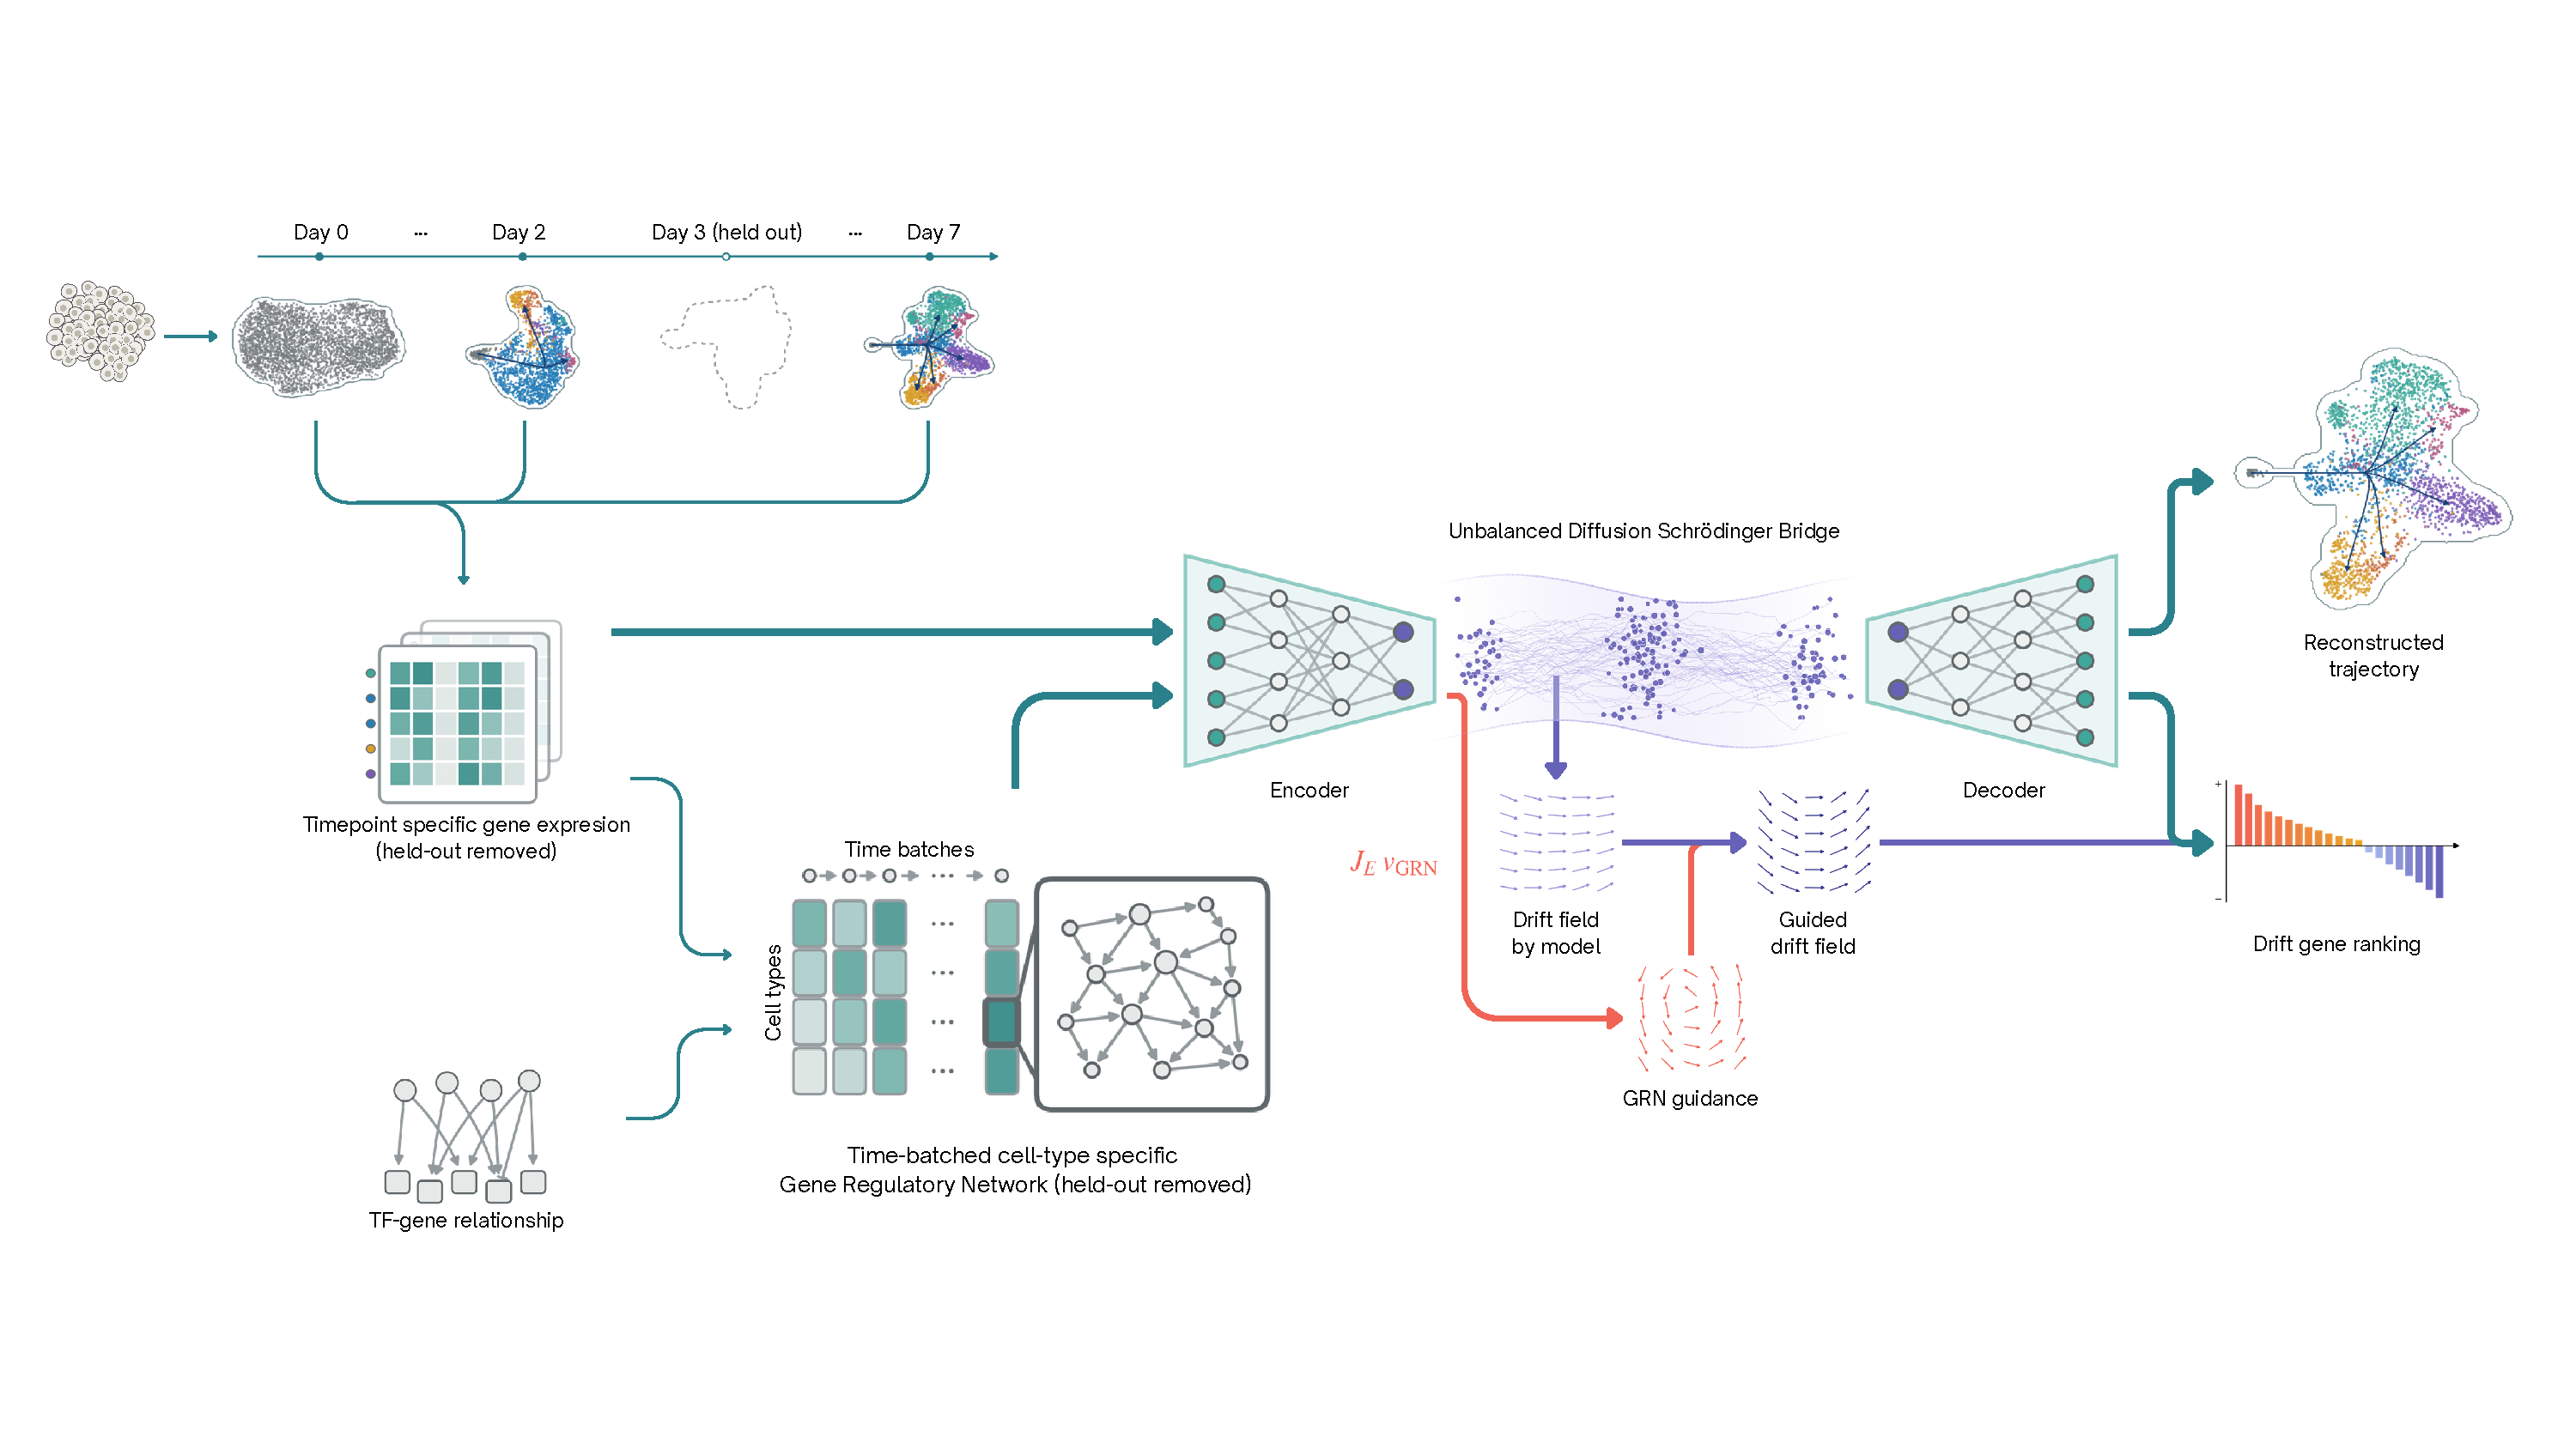
\includegraphics[width=\textwidth,trim=20pt 112pt 25pt 114pt,clip,keepaspectratio,alt={Overview of GRASB. A cell-contextualized regulatory velocity is mapped through the frozen VAE encoder to guide the latent drift, which is subsequently mapped through the frozen decoder for gene-resolved interpretation.}]{figures/grasb_main_figure.pdf}
\caption{Overview of GRASB. A cell-contextualized
regulatory velocity is mapped through the frozen VAE encoder to guide
the latent drift, which is subsequently mapped through the frozen
decoder for gene-resolved interpretation.}
\end{figure}

\subsection{3.2 VAE-based denoising and dimensionality
reduction}\label{vae-based-denoising-and-dimensionality-reduction}

We first learn the latent representation. The VAE encoder
\(q_\phi(z\mid x)=\mathcal{N}(\mu_\phi(x),\operatorname{diag}\sigma_\phi^2(x))\)
and decoder \(D_\psi:\mathbb{R}^{d}\rightarrow\mathbb{R}^{G}\) are
trained by minimizing

\[
\mathcal{L}_{\mathrm{VAE}}
=\mathbb{E}_{q_\phi(z\mid x)}\!\left[\lVert x-D_\psi(z)\rVert_2^2\right]
+\beta_{\mathrm{VAE}}\,D_{\mathrm{KL}}\!\left(q_\phi(z\mid x)\,\|\,\mathcal{N}(0,I)\right).
\]

After training, the bridge uses the posterior mean
\(E(x)=\mu_\phi(x)\). The VAE is time-independent, trained only on the
training timepoints, and then frozen so that every bridge condition,
simulation, and readout uses the same gene-to-latent mapping.

To place the latent features on comparable scales, we standardize them
using the training cells only. With training-set mean \(m_z\) and
standard deviation \(r_z\), the bridge state is

\[
z'=S(E(x))=\frac{E(x)-m_z}{r_z},
\qquad
S^{-1}(z')=m_z+r_z\odot z'.
\]

Thus \(\widetilde D(z')=D_\psi(S^{-1}(z'))\).

\subsection{3.3 Latent unbalanced diffusion Schrödinger
bridge}\label{latent-unbalanced-diffusion-schruxf6dinger-bridge}

\subsubsection{3.3.1 Schrödinger-bridge
transport}\label{schruxf6dinger-bridge-transport}

For endpoint distributions \(\mu_0\) and \(\mu_1\), an SB seeks the path
measure \(P^*\) closest in relative entropy to a reference diffusion
\(R\), subject to the prescribed marginals:

\[
P^*=\operatorname*{arg\,min}_{P}\;D_{\mathrm{KL}}(P\,\|\,R)
\quad\text{such that}\quad P_0=\mu_0,\;P_1=\mu_1.
\]

A diffusion SB learns neural forward and reverse drifts by alternating
IPF regressions on simulated paths \parencite{de_bortoli_diffusion_2021}. For a live
particle, the forward process is

\[
dZ_s=b_\theta(Z_s,s)\,ds+g(s)\,dW_s,
\qquad
b_\theta(z,s)=f(z,s)+g(s)U_\theta(z,s),
\]

where \(W_s\) is Brownian motion, \(f\) and \(g\) define the reference
diffusion, and \(U_\theta\) is a learned control. Forward and reverse
controls use scalar-potential networks as in uDSB-F and ARTEMIS
\parencite{pariset_unbalanced_2023,alatkar_artemis_2025}.

For simulated increment \(\Delta Z_k\) over \(\Delta s\), the forward
mean-matching loss is

\[
\mathcal{L}_{\mathrm{MM}}(\theta)
=\mathbb{E}\!\left[
\left\lVert\Delta Z_k-b_\theta(Z_{s_k},s_k)\Delta s\right\rVert_2
\right],
\]

with an analogous loss for the reverse-time drift.

\subsubsection{3.3.2 Unbalanced mass
dynamics}\label{unbalanced-mass-dynamics}

The balanced construction above cannot represent changes in population
size. To add this capability, uDSB-F augments
\(\mathbb{R}^{d}\) with a coffin state: forward killing becomes birth
under time reversal \parencite{pariset_unbalanced_2023}. Observed cell counts define
relative masses, and a neural killing-rate correction is trained with
the Ferryman loss to match cumulative birth and death at intermediate
checkpoints, following ARTEMIS \parencite{alatkar_artemis_2025}. The killing-rate
model is optimized jointly with the bridge; drift and regulatory losses
include only live particles.

\subsection{3.4 Cell-contextualized regulatory velocity in gene
space}\label{cell-contextualized-regulatory-velocity-in-gene-space}

We next construct the gene-space velocity used to guide the bridge. It
combines a fixed candidate topology with context-specific signed
coefficients.

\subsubsection{3.4.1 Regulatory topology and coefficient
estimation}\label{regulatory-topology-and-coefficient-estimation}

For each species, a promoter-supported TF--target map defines a binary
mask \(M\), restricted to modeled genes and excluding self-edges
\parencite{kamimoto_dissecting_2023}. It specifies candidate, not established causal,
regulation.

Within this shared topology, context \(c\) combines a cell-type or
lineage label with an interval between training timepoints. For target \(g\), let
\(\mathcal P_g=\{j:M_{gj}=1\}\). Target and regulator expression are
centered within each endpoint, yielding \(\widetilde y_{g,c}\) and
\(\widetilde X_{\mathcal P_g,c}\), and coefficients are estimated by

\[
\widehat\beta_{g,c}
=\operatorname*{arg\,min}_{\beta}
\left\lVert
\widetilde y_{g,c}-\widetilde X_{\mathcal P_g,c}\beta
\right\rVert_2^2
+\alpha_{g,c}\left\lVert\beta-\beta_{g,0}\right\rVert_2^2,
\qquad
\alpha_{g,c}=\alpha_0\left(1+\frac{|\mathcal P_g|}{n_c}\right),
\]

where \(n_c\) is the context size and \(\beta_{g,0}\) is a training-only
pooled estimate from the same lineage when sufficiently represented, or
otherwise from the interval. The adaptive shrinkage stabilizes small
contexts. Fits use only the two training endpoints; held-out
times are excluded. Contexts with fewer than 30 cells receive no
regulatory constraint.

The fitted coefficients define a sparse signed matrix
\(A_c\in\mathbb{R}^{G\times G}\):

\[
(A_c)_{gj}
=
\begin{cases}
(\widehat\beta_{g,c})_j, & j\in\mathcal P_g,\\
0, & j\notin\mathcal P_g.
\end{cases}
\]

Thus, the candidate topology is shared across contexts, while both the
fitted coefficients and the expression state are context dependent.

\subsubsection{3.4.2 Regulon velocity}\label{regulon-velocity}

For a gene-expression state \(x\) assigned to context \(c\), the
deployed regulatory velocity is

\[
v_{\mathrm{GRN}}^x(x,c)=\gamma_c A_cx.
\]

Genes without fitted target rows receive zero velocity. Define the raw
calibration velocity as \(q_c(x)=A_cx\). For represented targets
\(\mathcal C_c\), the positive scale \(\gamma_c\) matches its mean
magnitude to the observed rate of change between interval endpoints:

\[
V_{\mathrm{obs},c}
=\frac{
\left\lVert
\overline x_{\tau_c^+,\mathcal C_c}-\overline x_{\tau_c^-,\mathcal C_c}
\right\rVert_2
}{\tau_c^+-\tau_c^-},
\qquad
V_{\mathrm{raw},c}
=\frac{1}{|\mathcal S_c|}
\sum_{i\in\mathcal S_c}
\left\lVert q_c(x_i)_{\mathcal C_c}\right\rVert_2,
\]

where \(\mathcal S_c\) is the training-cell calibration set for context
\(c\). We set

\[
\gamma_c=\frac{V_{\mathrm{obs},c}}{V_{\mathrm{raw},c}},
\]

and fix this value before bridge training. The resulting velocity is an
observational soft prior; its coefficient signs describe associations
rather than established causal effects.

\subsection{3.5 Regulatory guidance and gene-resolved
interpretation}\label{regulatory-guidance-and-gene-resolved-interpretation}

\subsubsection{3.5.1 Mapping regulatory velocity to latent
space}\label{mapping-regulatory-velocity-to-latent-space}

The regulatory velocity must now be compared with a drift learned in
latent space. At latent state \(z'\), let
\(\widehat x=\widetilde D(z')\). We transport the gene-space velocity as
a tangent vector through the encoder:

\[
v_{\mathrm{GRN}}^z(z',s,c)
=J_{S\circ E}(\widehat x)\,v_{\mathrm{GRN}}^x(\widehat x,c)
=\operatorname{diag}(r_z^{-1})J_E(\widehat x)
  v_{\mathrm{GRN}}^x(\widehat x,c).
\]

This and subsequent products are evaluated as JVPs without materializing
Jacobians.

Before applying the penalty, we convert velocity from developmental time
to normalized time by multiplying it by \(\tau_M-\tau_0\), assign each
bridge step to its developmental interval, and carry the source cell
label along the path. Missing or unlabeled contexts receive no penalty.

The primary training objective is

\[
\mathcal{L}_{\mathrm{total}}
=\mathcal{L}_{\mathrm{MM}}
+\lambda_{\mathrm{GRN}}\mathcal{L}_{\mathrm{GRN}}
+\mathcal{L}_{\mathrm{mass}},
\]

where \(\mathcal{L}_{\mathrm{mass}}\) denotes the Ferryman mass-matching
terms and

\[
\mathcal{L}_{\mathrm{GRN}}
=\mathbb{E}_{(Z_s,c)\,\mid\,\mathrm{alive}}
\left[
\left\lVert b_\theta(Z_s,s)-v_{\mathrm{GRN}}^z(Z_s,s,c)\right\rVert_2^2
\right].
\]

Setting \(\lambda_{\mathrm{GRN}}=0\) gives the matched latent uSB
baseline.

\subsubsection{3.5.2 Mapping learned dynamics to gene
space}\label{mapping-learned-dynamics-to-gene-space}

The inverse readout uses the same fixed representation. After training,
the decoder differential maps the forward latent drift back to gene
space. For a latent state \(z'\),

\[
b_\theta^x(z',s)
=J_{D_\psi}(S^{-1}(z'))\,\operatorname{diag}(r_z)b_\theta(z',s)
=J_{\widetilde D}(z')b_\theta(z',s).
\]

Its components are local signed gene-expression rates. We average them
within each eligible lineage and time before ranking genes. Generated
expression is evaluated separately by simulating from a source marginal
and decoding the terminal states; it accumulates drift, diffusion, and
birth/death rather than measuring the local vector field.

\subsection{3.6 Matched controls}\label{matched-controls}

To distinguish topology-specific guidance from generic regularization,
we compare the genuine-GRN condition with two matched controls. The
no-GRN baseline sets \(\lambda_{\mathrm{GRN}}=0\). The shuffled-GRN
control preserves each target's number of incoming edges, fitted
coefficient values, context structure, and scale factor, but reassigns
its regulators from the same TF pool while excluding self-regulation.
The same reassignment is used across contexts. The shuffle therefore
preserves the sparsity and coefficient distribution of the guidance term
while disrupting TF--target identity. All three conditions use the same
preprocessing, frozen VAE, uSB, mass-model architecture, and
optimization settings; the bridge is trained independently for each
condition.

\section{4. Evaluation and results}\label{evaluation-and-results}

\subsection{4.1 Experimental design and evaluation
criteria}\label{experimental-design-and-evaluation-criteria}

We evaluated held-out intermediate timepoints in stage-5 human
pancreatic differentiation \parencite{veres_charting_2019} and zebrafish
embryogenesis from 3.3 to 12 hours post fertilization (hpf)
\parencite{farrell_single-cell_2018}. Pancreatic days 3 and 6 and zebrafish 5.3, 7, and 9 hpf were
excluded from VAE, bridge, and GRN fitting. The primary zebrafish
analysis used 7 and 9 hpf; 5.3 hpf was reserved for sensitivity analysis
because its adjacent source contained fewer than 40 cells in two target
lineages. Within each context, the genuine and shuffled arms used the
same pre-calibrated \(\gamma_c\). Model configurations and shared
hyperparameters are summarized in Table~\ref{tab:model-configurations}.

\begin{table}[H]
\caption{Model configurations and hyperparameters in the two
developmental systems.}
\label{tab:model-configurations}

\begin{center}
\begin{tabularx}{\textwidth}{@{}>{\raggedright\arraybackslash}p{0.27\textwidth}
  >{\centering\arraybackslash}X >{\centering\arraybackslash}X@{}}
\toprule
 & pancreatic differentiation & zebrafish embryogenesis \\
\midrule
VAE KL weight, \(\beta_{\mathrm{VAE}}\) & 0.3 & 0.3 \\
guidance weight, \(\lambda_{\mathrm{GRN}}\) & 1 & 0.03 \\
\midrule
matched arms & \multicolumn{2}{c}{no GRN, genuine GRN, degree-preserving topology shuffle} \\
latent representation & \multicolumn{2}{c}{10-dimensional frozen VAE} \\
reference process & \multicolumn{2}{c}{zero drift; triangular diffusion, \(g_{\max}=0.5\)} \\
numerical integration & \multicolumn{2}{c}{100 Euler-Maruyama steps} \\
bridge architecture & \multicolumn{2}{c}{hidden width 512} \\
optimization & \multicolumn{2}{c}{batch size 512; learning rate \(10^{-4}\)} \\
training schedule & \multicolumn{2}{c}{six phases; ten epochs per phase} \\
trajectory updates & \multicolumn{2}{c}{ten per direction and epoch} \\
path-batch reuse & \multicolumn{2}{c}{five updates per simulated batch} \\
\bottomrule
\end{tabularx}
\end{center}
\end{table}

We evaluate the two model outputs separately. Decoded-drift metrics test
whether the local vector field prioritizes an expected lineage program.
Wasserstein-2 distance (W2), for which lower is better, instead compares
generated and observed held-out populations after integrating the
stochastic dynamics. The two evaluations therefore measure local
biological organization and population reconstruction, respectively.

\FloatBarrier
During model development, expression specificity proved insufficient on
its own: a latent no-GRN model could produce lineage-specific expression
signatures without recovering canonical markers. We therefore based the
final evaluation on predefined gene sets and topology shuffles.

Pancreatic sets were the positive identity markers from \textcite{veres_charting_2019},
and zebrafish sets mapped the six-somite modules from \textcite{farrell_single-cell_2018} to
terminal lineages. Because
these sets define expressed lineage identities rather than repressed
programs, primary analyses used positive drift. GSEA normalized
enrichment score (NES) evaluated each set against the complete signed
drift ranking \parencite{subramanian_gene_2005}. Recall@\(K\) measured the
fraction recovered among the strongest positive-drift genes
(\(K=15\) for pancreas; \(K=50\) for the broader zebrafish modules).
Scoring every eligible lineage set against each ranking also tested
whether the matching program ranked above alternatives.

\subsection{4.2 Lineage-marker recovery through genuine GRN
topology}\label{lineage-marker-recovery-through-genuine-grn-topology}

We first evaluated pancreatic differentiation. Genuine GRN guidance
improved both marker-set enrichment and individual-marker recovery over
no GRN and all six shuffled topologies
(Table~\ref{tab:pancreas-results}).

\begin{table}[H]
\caption{Pancreatic lineage-marker recovery and held-out population
reconstruction.}
\label{tab:pancreas-results}

\begin{center}
\begin{tabularx}{\textwidth}{@{}>{\raggedright\arraybackslash}X
  >{\centering\arraybackslash}p{0.15\textwidth}
  >{\centering\arraybackslash}p{0.18\textwidth}
  >{\centering\arraybackslash}p{0.24\textwidth}@{}}
\toprule
 & no GRN & genuine GRN & shuffled GRN \\
\midrule
GSEA NES for the matching marker set & 0.053 & \textbf{1.260} & \mbox{\(-0.158 \pm 0.241\)} \\
marker recall@15 & 9.4\% & \textbf{31.9\%} & \mbox{\(10.5 \pm 5.4\%\)} \\
W2, day 3 & \textbf{10.513} & 11.151 & \mbox{\(11.279 \pm 0.176\)} \\
W2, day 6 & \textbf{8.942} & 10.923 & \mbox{\(10.937 \pm 0.051\)} \\
\bottomrule
\end{tabularx}
\end{center}

* For GSEA NES and marker recall@15, higher values are better; for W2,
lower values are better. Shuffled-GRN values are mean \(\pm\) SD across
six fixed randomized topologies.
\end{table}

The improvement was substantial: genuine guidance increased NES from
0.053 to 1.260 and recall@15 from 9.4\% to 31.9\%.
Degree-preserving shuffles returned recall near the
unguided level and produced negative mean NES, showing that the gain
depended on regulatory edge identity. The matching marker set also
ranked 2.89 on average, versus 5.27 after within-stage label permutation
(one-sided \(p=0.0002\)), indicating lineage-specific rather than global
enrichment.

At the gene level, genuine guidance raised the positive-drift ranks of
\emph{NEUROG3}, \emph{PAX4}, and \emph{FEV} in endocrine progenitor
states, as well as \emph{SST}, \emph{ARX}, and \emph{DDC} in later
endocrine states. These genes were expressed in their matched observed
populations (Figure~\ref{fig:grn-guided-gene-ranks-expression}a,c),
consistent with the lineage-specific marker-program enrichment.

\FloatBarrier
\subsection{4.3 Context-specific coefficient
swapping}\label{context-specific-coefficient-swapping}

To test whether the fitted coefficients were interchangeable across
states, we reassigned coefficient sets while keeping the common
topology. From the lowest to highest quartile of expression divergence,
marker recall for the evaluated state fell from 0.140 to 0.026, and the
fraction of signatures matching neither the evaluated nor coefficient
origin lineage rose from 63\% to 87\%. Thus, swapping coefficients
between similar states preserved more of the original signal, whereas
swaps between divergent states increasingly disrupted lineage-specific
drift.

\subsection{4.4 Lineage-module recovery in zebrafish
embryogenesis}\label{lineage-module-recovery-in-zebrafish-embryogenesis}

We next asked whether the pancreatic result generalized to zebrafish.
Using the lineage modules of \textcite{farrell_single-cell_2018}, genuine guidance
again improved agreement over both controls
(Table~\ref{tab:zebrafish-results}). These sets
contained 21--51 genes, including 11--34 lineage-specific genes.

Across all three paired seeds, genuine GRN improved NES, recall@50, and
matching-module rank over both controls. The advantage arose mainly at 9
hpf; at 7 hpf, the frozen VAE already supported strong module-aligned
drift without guidance.

At the gene level, genuine guidance elevated somitic, adaxial, and axial
mesoderm genes that the no-GRN model under-prioritized, including
\emph{RIPPLY1}, \emph{CDKN1CA}, \emph{MYOD1}, \emph{PCDH8}, \emph{TA},
and \emph{TBX16} (Figure~\ref{fig:grn-guided-gene-ranks-expression}b).
Observed expression placed these genes in the corresponding somitic,
adaxial, or axial mesoderm populations
(Figure~\ref{fig:grn-guided-gene-ranks-expression}d), matching the
lineage assignments used for evaluation.

\begin{figure}[!tbp]
\centering
\makebox[\textwidth][c]{%
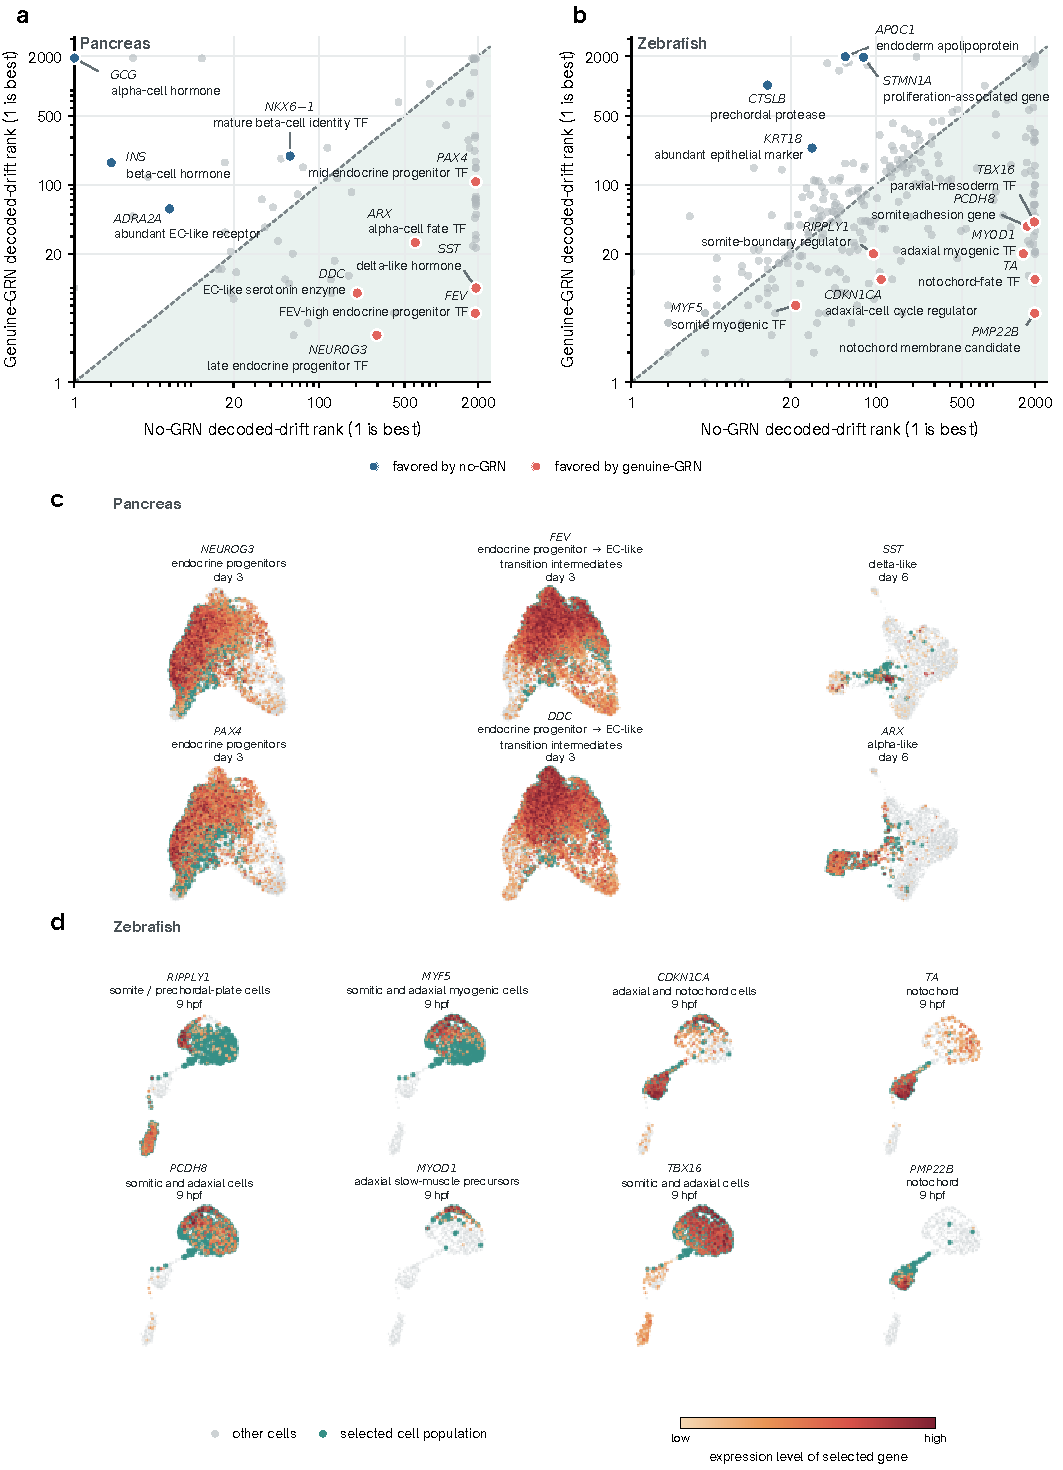
\includegraphics[width=1.06\textwidth,height=0.86\textheight,trim=2pt 3pt 6pt 3pt,clip,keepaspectratio]{figures/figure2_combined_v2.pdf}%
}
\caption{\textbf{GRN guidance reprioritizes lineage-relevant decoded
drift.} Gene-rank comparisons show regulatory or lineage-program genes
promoted from weaker no-GRN ranks and prominent output or
state-associated genes shifted to weaker ranks by genuine guidance
(a,b). Observed expression of guidance-promoted genes is shown in the
matched cell populations (c,d).}
\label{fig:grn-guided-gene-ranks-expression}
\end{figure}

\begin{table}[H]
\caption{Zebrafish decoded-drift results at the primary 7 and 9 hpf
targets.}
\label{tab:zebrafish-results}

\begin{center}
\begin{tabularx}{\textwidth}{@{}>{\raggedright\arraybackslash}X
  >{\centering\arraybackslash}p{0.19\textwidth}
  >{\centering\arraybackslash}p{0.19\textwidth}
  >{\centering\arraybackslash}p{0.19\textwidth}@{}}
\toprule
 & no GRN & genuine GRN & shuffled GRN \\
\midrule
GSEA NES for the matching lineage module & \mbox{\(1.106 \pm 0.247\)} & \mbox{\(\mathbf{1.622 \pm 0.044}\)} & \mbox{\(0.711 \pm 0.336\)} \\
marker recall@50 & \mbox{\(0.365 \pm 0.064\)} & \mbox{\(\mathbf{0.503 \pm 0.017}\)} & \mbox{\(0.299 \pm 0.066\)} \\
rank of the matching lineage module & \mbox{\(2.370 \pm 0.178\)} & \mbox{\(\mathbf{1.615 \pm 0.340}\)} & \mbox{\(3.356 \pm 0.550\)} \\
W2, 7 hpf & \mbox{\(\mathbf{14.644 \pm 1.243}\)} & \mbox{\(16.891 \pm 1.329\)} & \mbox{\(16.284 \pm 1.703\)} \\
W2, 9 hpf & \mbox{\(\mathbf{15.376 \pm 0.847}\)} & \mbox{\(18.301 \pm 1.808\)} & \mbox{\(17.963 \pm 1.652\)} \\
\bottomrule
\end{tabularx}
\end{center}

* Higher values are better for GSEA NES and marker recall@50; lower
values are better for module rank and W2. Values are mean \(\pm\) SD
across three independently trained models.
\end{table}

\subsection{4.5 Regulatory reprioritization of an expression-informed
baseline}\label{regulatory-reprioritization-of-an-expression-informed-baseline}

The rank comparison in Figure~\ref{fig:grn-guided-gene-ranks-expression}
shows that the no-GRN model was not devoid of biological information.
It assigned strong ranks to prominent terminal products and
state-associated genes, including \emph{GCG}, \emph{INS}, \emph{ADRA2A},
and \emph{NKX6-1} in pancreas and \emph{APOC1}, \emph{STMN1A},
\emph{CTSLB}, and \emph{KRT18} in zebrafish. These genes indicate that
the frozen VAE supplied an expression-informed baseline capable of
recognizing conspicuous features of the observed state.

The expression-aligned analysis in
Figure~\ref{fig:pancreas-expression-aligned-drift-ranks} clarifies the
limitation of that baseline. Without GRN guidance, decoded drift often
favored terminal products or state markers such as \emph{INS},
\emph{GCG}, and \emph{CALB2}, which were highly expressed in their
matched populations. This was valid lineage information, but it was
weighted toward genes already prominent in the observed state.

The relationship was not a simple mapping from mean expression to rank.
Visibly expressed regulatory or lineage-associated genes, including
\emph{FEV}, \emph{DDC}, and \emph{NEUROD1}, remained comparatively weak
without guidance, while the genuine-GRN model elevated \emph{NEUROG3},
\emph{CDKN1C}, \emph{MAFB}, and \emph{ARX}. Conversely, \emph{SCG5},
\emph{ACVR1C}, \emph{SLC30A8}, \emph{GAL}, and \emph{SCG2} received
meaningful ranks from both models. The no-GRN failure mode was therefore
incomplete regulatory attribution, rather than absent lineage signal or
deterministic ranking by expression abundance. Together,
Figures~\ref{fig:grn-guided-gene-ranks-expression}
and~\ref{fig:pancreas-expression-aligned-drift-ranks} show that genuine
GRN guidance reorganizes an expression-informed baseline toward
regulatory and lineage-program genes that it otherwise under-prioritizes.

\begin{figure}[!tbp]
\centering
\makebox[\textwidth][c]{%
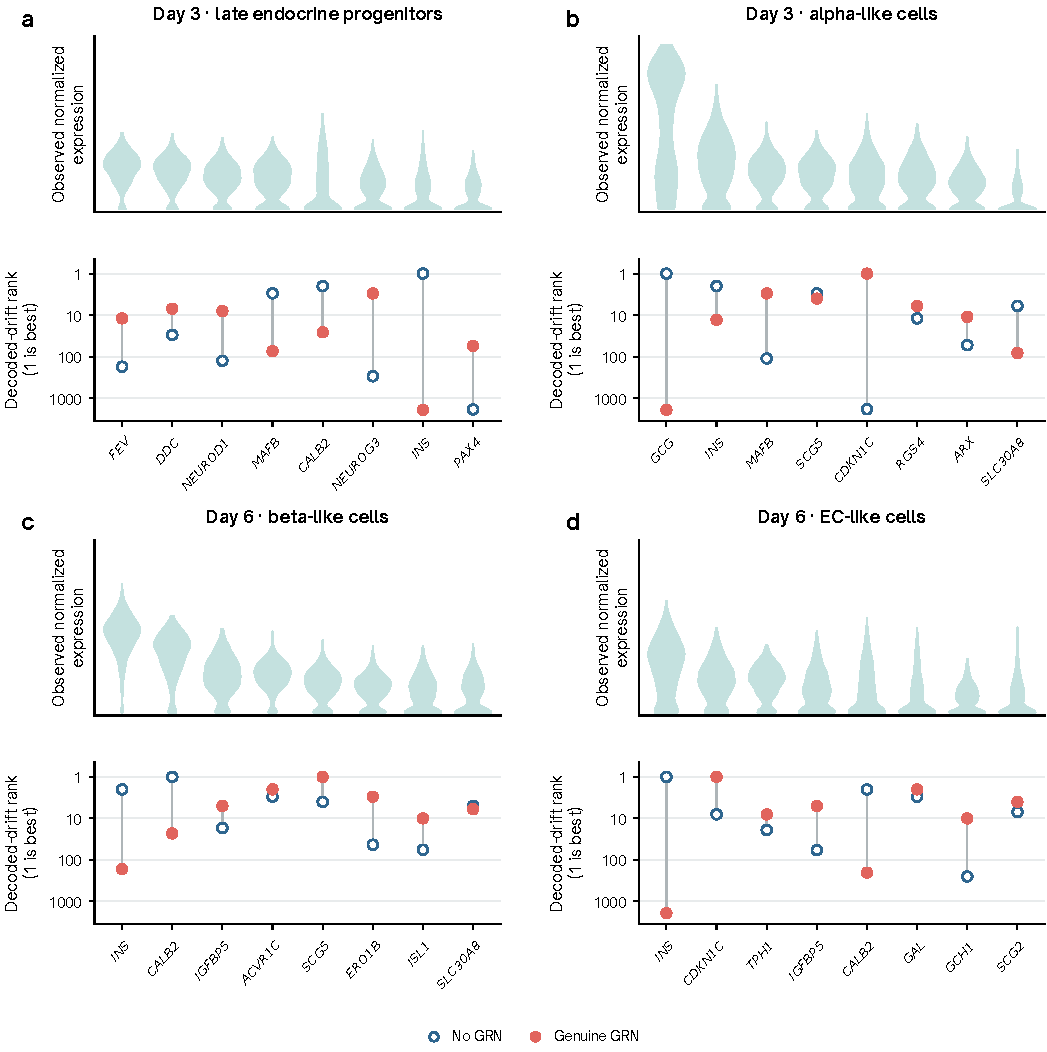
\includegraphics[width=0.94\textwidth,height=0.74\textheight,keepaspectratio]{figures/figure3_pancreas_ranked_violins_v1.pdf}%
}
\caption{\textbf{Expression-aligned ranks expose incomplete regulatory
attribution without GRN guidance.} Across four pancreatic lineage--day
settings, no-GRN drift favors highly expressed output or state-marker
genes while assigning weak ranks to several expressed regulators.
Genuine guidance elevates those regulators; genes ranked strongly by
both models show that the failure is incomplete regulatory attribution,
not loss of lineage signal.}
\label{fig:pancreas-expression-aligned-drift-ranks}
\end{figure}

\subsection{4.6 Trade-off between decoded-drift interpretation and reconstruction
fidelity}\label{trade-off-between-decoded-drift-interpretation-and-reconstruction-fidelity}

This improvement in local drift did not translate into better population
reconstruction. In both systems, improved marker or module recovery
coincided with higher held-out W2 (Tables~\ref{tab:pancreas-results}
and~\ref{tab:zebrafish-results}). Genuine and shuffled GRNs had
similar W2 despite different biological recovery. In the pancreatic
dataset, varying \(\lambda_{\mathrm{GRN}}\) from 0.25 to 2 did not recover
the distributional fidelity of the no-GRN model; most of the loss
occurred at the smallest nonzero weight. Under these
settings, imposing a nonzero local-vector-field constraint was the main
source of the trade-off between drift interpretation and population
reconstruction, rather than the GRN topology or the precise guidance
weight.

\FloatBarrier
\section{5. Discussion and
limitations}\label{discussion-and-limitations}

GRASB couples gene-resolved regulatory information to
latent stochastic transport without redefining the GRN over unnamed
variables in the latent representation. The cell-contextualized GRN remains in gene space,
where TF and target identities are preserved; an encoder JVP transports
its velocity into the frozen VAE representation, and a decoder JVP
returns the learned drift to signed velocities for named genes. Freezing
the VAE makes this mapping stable across experimental conditions. The
framework therefore combines the denoising and computational advantages
of latent transport with a gene-level regulatory reference that can be
directly tested.

The topology-controlled evaluation shows that this guidance changes the
biological attribution of local drift. The frozen VAE baseline already
recognized terminal identity genes and part of the shared lineage signal;
genuine GRN guidance reorganized that signal toward regulatory and
lineage-program genes that the baseline under-prioritized. This advantage
was lost after degree-preserving edge shuffling, and fitted regulatory
weights transferred best between transcriptionally similar states.
Although this reprioritization is not a causal claim, it supports a
specific interpretation: the GRN prior organizes the learned vector
field toward known lineage programs through both regulatory edge identity
and cellular context.

The results also separate vector-field interpretation from trajectory
reconstruction. Guidance improved marker
and module recovery but increased held-out W2, while genuine and shuffled
GRNs produced similar W2 despite markedly different biological recovery.
This pattern suggests that constraining the drift caused most of the
fidelity loss, whereas genuine topology supplied the biological benefit.
Consequently, distributional fit alone is insufficient when a trajectory
model is used for gene-level interpretation, but marker alignment alone
is also insufficient when accurate population generation is required.
Applications should report both outcomes, select the guidance strength
using training data or nested validation, and include a
degree-preserving shuffled-GRN control to test whether interpretation
depends on regulatory topology.

Several limitations bound these conclusions. We evaluated two
developmental systems and one GRN-construction procedure based on
observational expression and promoter-supported candidate edges. This
prior does not capture distal enhancer activity, chromatin accessibility,
or dynamic network rewiring; SCENIC+ and Dictys, along with CellOracle
discussed above, provide important alternatives
\parencite{bravo_gonzalez-blas_scenic_2023,wang_dictys_2023,kamimoto_dissecting_2023}. For each system, the cell
labels and marker sets came from one source study, tying evaluation to
that study's definitions of cell identity. Comparisons across independent annotations, regulatory
priors, and datasets are therefore needed to establish generality.

Measured perturbation responses provide the clearest next test of whether
decoded drift predicts regulatory change. Time-resolved genetic or drug
perturbations could evaluate response direction and heterogeneous
trajectories, including the emergence of resistant states. Neural OT has
already modeled single-cell drug responses from unpaired control and
treated populations \parencite{bunne_learning_2023}, providing a relevant
comparison. Extending the present framework to perturbation-conditioned
transport would move the analysis from alignment with known
developmental programs toward experimentally testable predictions of
regulatory response.

\printbibliography[heading=bibintoc,title={References}]

\end{document}
